\documentclass{report}
\usepackage{pdfpages}
\usepackage{pgf,tikz}
\usetikzlibrary{arrows}

\begin{document}
\thispagestyle{empty}
\begin{center}
{\Huge Transactions\\ in\\[.2in] \textbf{Euclidean Geometry}}
\vspace{1in}

\begin{figure}[h!]
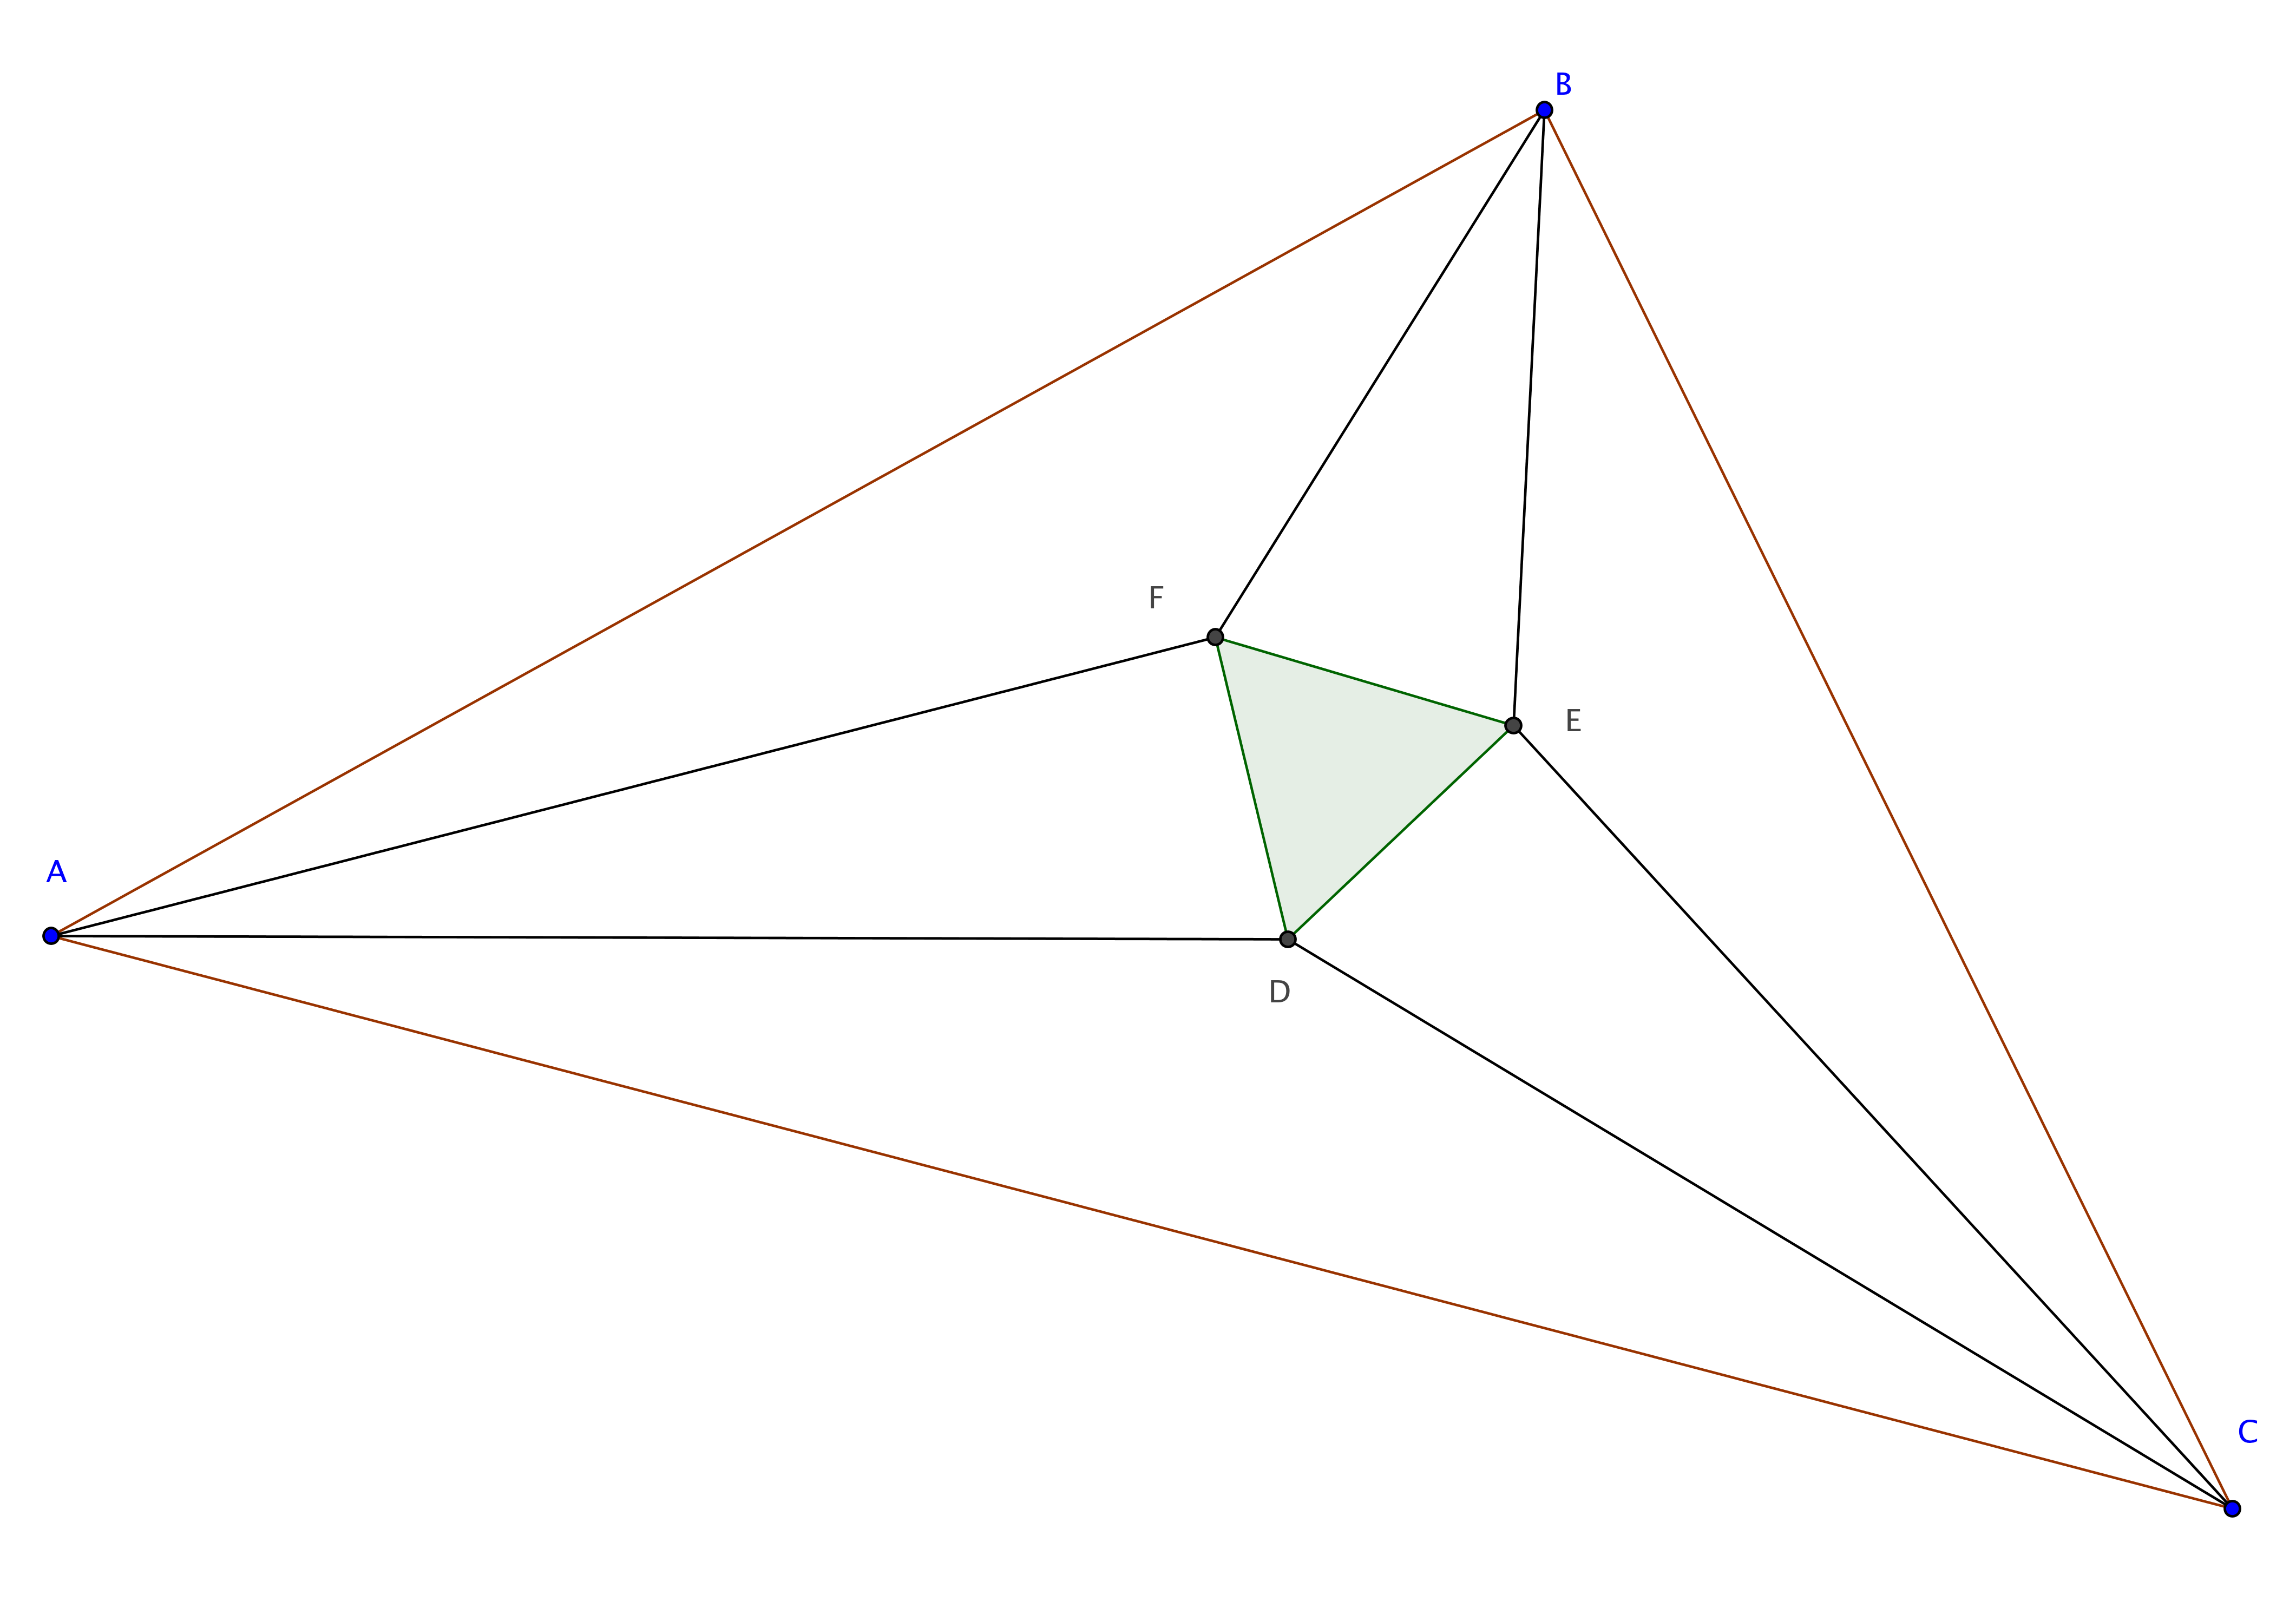
\includegraphics[width=1.1\textwidth]{cover-image.png}
\end{figure}

\vspace{.5in}

{\Large Volume 2020S}\\[.25in]
{\Huge Issue \# 7}
\end{center}

\clearpage

\center \Large \textbf{Table of Contents}\\[.25in]
\normalsize
\begin{tabular}{lr}
\textbf{Title} & \textbf{Author}\\[.25in]
\emph{Pairs of Opposite in a Kite} & Brad Warner \\
\hspace{.1in}\emph{are Congruent} \\[.25in]
\emph{Finding the Parallel Line} & Jimmy Pham \\[.25in]
\emph{Finding the Parallel Line, Part II} & Jimmy Pham \\[.25in]
\emph{Squares Inscribed in a Triangle} & Payson VandeLune \\
  & \& Lexis Wiegmann\\[.25in]
%\emph{A Kite is Not a Parallelogram} & Lexis Wiegmann\\[.25in]
%\emph{Convex vs. Non-Convex Quadrilaterals} & Lexis Wiegmann \\[.25in]
%\emph{Parallel and Perpendicular Lines} & Alexa DeVore \\[.25in]
%\emph{Angle Bisector Concurrence} & Payson VandeLune \\[.25in]
%\emph{Stine's ASS Theorem} & Jason Stine\\[.25in]
%\emph{Construction of an Equilateral Pentagon} & Lauren Falck\\[.25in]
%\emph{Construction of a Regular Pentagon} & Lauren Falck \\[.25in]
%\emph{Angles within a Circle} & Jacklyn Miller \\[.25in]
%\emph{Proving HL using Pythagoras} & Jason Stine \\[.25in]
%\emph{Squaring a Rectangle} & Payson VandeLune \\
%    & \& Jaclyn Miller \\[.25in]
%\emph{Tangent Line of a Circle} & Lexis Wiegmann \\[.25in]
\end{tabular}

\includepdf[pages=-]{1.pdf}
\includepdf[pages=-]{2.pdf}
\includepdf[pages=-]{3.pdf}
\includepdf[pages=-]{4.pdf}
%\includepdf[pages=-]{5.pdf}
%\includepdf[pages=-]{6.pdf}
%\includepdf[pages=-]{7.pdf}
%\includepdf[pages=-]{8.pdf}
%\includepdf[pages=-]{9.pdf}
%\includepdf[pages=-]{10.pdf}
%\includepdf[pages=-]{11.pdf}
%\includepdf[pages=-]{12.pdf}
%\includepdf[pages=-]{13.pdf}
%\includepdf[pages=-]{14.pdf}
%\includepdf[pages=-]{15.pdf}




\end{document}